\section{Introduction}\label{sec:introduction}

For a finite graph \(G\), write \(\alpha(G)\), \(\chi(G)\), and \(h(G)\)
for its independence number, chromatic number, and Hadwiger number.
Thus \(h(G)\) is the largest \(t\) for which \(G\) contains a \(K_t\)
minor.

Hadwiger's conjecture, formulated in 1943~\citep{hadwiger1943},
asserts that \(h(G)\ge\chi(G)\) for every finite nonempty simple
graph \(G\). We disprove it using graphs of independence number
at most 2.

Two disjoint edges are \emph{touching} if an edge joins their
endpoint sets. A \emph{connected matching} is a matching whose edges
are pairwise touching. Write \(\cm(G)\) for the maximum size of a connected matching in \(G\).

% lax begin Lax793645.Counterexample
\begin{theorem}\label{thm:main}
There are arbitrarily large integers \(m\) for which an \(m\)-vertex
finite simple graph \(G\) satisfies
\[
             \alpha(G)\le2
             \qquad\text{and}\qquad
             \cm(G)<\frac{m}{100}.
\]
\end{theorem}
% lax end

The connection to minors comes from the small branch sets of a
\(K_t\) minor. Its branch sets of size 2 form a connected matching,
and pairing its singleton branch sets gives more edges in the same
matching. Counting the vertices in the remaining branch sets gives
\[
                    h(G)\le\frac{|V(G)|+4\cm(G)+2}{3}
\]
(Proposition~\ref{prop:matching-minor}).

It is enough to compare this upper bound with the fractional chromatic
number. Write \(\mathcal I(G)\) for the independent sets of \(G\).
A fractional coloring assigns each \(I\in\mathcal I(G)\) a weight
\(w_I\ge0\) such that \(\sum_{I\ni v}w_I\ge1\) at every vertex \(v\).
The minimum total weight is \(\chi_f(G)\). Giving weight 1 to each
color class of an ordinary coloring shows that \(\chi_f(G)\le\chi(G)\).

% lax begin Lax793645.FractionalCounterexample
\begin{corollary}\label{cor:hadwiger}\label{cor:fractional-hadwiger}
There are finite nonempty simple graphs \(G\) of arbitrarily large
order \(m\) for which
\[
 h(G)<\frac{26m}{75}+\frac23
 <\frac m2\le\chi_f(G)\le\chi(G).
\]
Thus Hadwiger's conjecture and its weakening to fractional colorings
\(\chi_f(G)\le h(G)\) are false.
\end{corollary}
% lax end
% lax begin Lax793645Proofs.FractionalCounterexample.arbitrarily_large_fractional_counterexample
\begin{proof}
Summing the vertex constraints of any fractional coloring gives
\[
 |V(G)|\le\sum_{I\in\mathcal I(G)}|I|w_I
       \le\alpha(G)\sum_{I\in\mathcal I(G)}w_I.
\]
Hence \(\chi_f(G)\ge |V(G)|/\alpha(G)\). Apply
\Cref{thm:main} and the minor bound above, noting that
\(26m/75+2/3<m/2\) for \(m\ge5\).
% lax begin Lax793645Proofs.Counterexample.arbitrarily_large_hadwiger_counterexample
Since \(\chi_f(G)\le\chi(G)\), the same graphs satisfy \(h(G)<\chi(G)\).
% lax end
\end{proof}
% lax end

\citet[p.~148]{reedseymour1998} discussed the conjecture that every graph with no
\(K_{p+1}\) minor has a fractional \(p\)-coloring and proved a
\(2p\) bound in their result (1.3). They require rational weights
and coverage exactly 1 at each vertex. Such weights satisfy the
constraints above, so taking \(p=h(G)\) also disproves their formulation.

\subsection{Context}

Hadwiger's conjecture was proposed in 1943~\citep{hadwiger1943}.
Its restriction to graphs with independence number at most 2 is equivalent
to the assertion that every such graph of order \(m\) has a
\(K_{\lceil m/2\rceil}\) minor~\citep[Theorem~3.1]{pst2003}.
The general bound of Duchet and Meyniel~\citep{duchet1982} gives a minor
of order at least \(m/3\) in this case. Our examples have Hadwiger number
less than \(26m/75+2/3\).

F\"uredi, Gy\'arf\'as, and Simonyi~\citep{fgs2005} conjectured that a graph
with independence number two and order \(4t-1\) has a connected matching
of size \(t\). \Cref{thm:main} disproves this statement as well. Delete
at most 3 vertices to obtain order \(4t-1\); the connected matching
number does not increase. The result does not assert that the matching
number is sublinear. It leaves open the possibility of a smaller universal
positive linear lower bound.

The proof below is an exposition of the construction in the accompanying
Lean submission. It does not use the separate counterexample based on the
Colin de Verdi\`ere invariant~\citep{OpenAIColinDeVerdiereCounterexample2026}.



\subsection{How the proof works}

We first define a symmetric relation on a finite set. We call a related
pair a \emph{hole}. To obtain a graph, sample \(m\) elements of the set
independently and join two distinct sample positions if there is no hole
between their elements. The relation has no loops, so two positions
carrying the same element are adjacent. A parity argument excludes
triangles of holes and hence independent sets of size 3.

Call an ordered pair with no internal hole a \emph{unit}. It represents
an edge of the sample graph. Two units \emph{conflict} if all four pairs
between them are holes. Edges of a connected matching cannot conflict.

\begin{figure}[htbp]
\centering
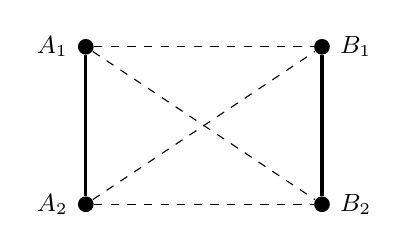
\begin{tikzpicture}[every node/.style={font=\small}]
\node[circle,fill=black,inner sep=2pt,label=left:$A_1$] (a1) at (0,1) {};
\node[circle,fill=black,inner sep=2pt,label=left:$A_2$] (a2) at (0,-1) {};
\node[circle,fill=black,inner sep=2pt,label=right:$B_1$] (b1) at (3,1) {};
\node[circle,fill=black,inner sep=2pt,label=right:$B_2$] (b2) at (3,-1) {};
\draw[very thick] (a1)--(a2); \draw[very thick] (b1)--(b2);
\draw[dashed] (a1)--(b1); \draw[dashed] (a1)--(b2);
\draw[dashed] (a2)--(b1); \draw[dashed] (a2)--(b2);
\end{tikzpicture}
\caption{The solid edges conflict when all four dashed pairs are holes.}
\label{fig:four-holes}
\end{figure}

Choosing an edge from a matching biases the choice of its endpoints.
A conflict estimate for four independent vertices would therefore be
insufficient. Theorem~\ref{thm:raw-supersaturation} gives a lower bound
for two independent units drawn from the same law. It allows dependence
within each unit and bounds how heavily its law can weight any vertex
or pair of vertices.

Here is how we witness a hole. Each raw vertex carries a linear
embedding on each edge of an auxiliary odd cycle. A point at a cycle
vertex has two images, one in each incident component. We call this
pair of images its \emph{key}. For each of the four proposed holes we
seek two short lists of points, one at either endpoint. If corresponding
keys agree, the sums of their point matrices have the same ambient
image. Further equations prescribe a linear functional on these sums.
We show that once the scalar equations hold, the remaining matrix
entries can be filled in without changing any images already fixed.

The lists at opposite ends of a hole are sampled independently before
we ask for their keys to agree. Such an equality is rare. To estimate
its probability we compare the two distributions of accepted keys.
Finite Fourier analysis lets us replace a distribution by its averages
on the cells of a partition given by linear equations. A character of
a tuple of keys factors into characters of its individual keys, so we
can test a whole list using information about individual points.

If the scalar equations have no solution, a linear relation determines
one of the recorded bits from the common key coordinates. This relation
holds for every point with those coordinates, which makes the prediction
an exact quadratic identity. When many units share a prediction, a
separate argument finds solutions on compatible pairs of units. Their
probability can be as small as order \(N^{-4}\). We bound the exceptional
probabilities under independent sampling before restricting to such pairs.

Finally, suppose every sample had a large connected matching. From each
matching select a short list of edges. With high probability it meets the set of
edges conflicting with any given unit whose conflicts occupy a substantial
fraction of the matching. Samples that supply
the same list then yield a law on edges under which two independent
draws conflict too rarely. This contradicts the lower bound.

\subsection{Conventions}

All vector spaces are over \(\F\). Probabilities and norms are real.
The polar form of \(q\) is \(\beta_q(v,w)=q(v+w)+q(v)+q(w)\).
We evaluate \(q\) on symmetric matrices by linearity, assigning
\(vv\trans\) the value \(q(v)\). These matrices span the symmetric
matrices.

The integer \(n\) tends to infinity. We write \(N=M_0n\) for the full
ambient dimension, with \(M_0\) a fixed even integer. The corresponding
dimension parameter in Lean is \(N/2\). All construction parameters are
fixed before \(n\). A bounded quantity is bounded independently of \(n\).

An \emph{orientation} specifies the two raw vertices of a unit in order.
At a fixed orientation a \emph{query} draws the parameters of its points.
We sometimes fix the images of prescribed directions, called \emph{pins}.
A \emph{leaf} carries the resulting conditional law together with the
images already fixed. In a mixture of leaves we retain the probability
of each leaf. Likewise, the measure of accepted keys has total mass equal
to the probability of acceptance.
